\section{Modelling mathematics}

TODO: Fix this paragraph
In order to program a neural network, I will first enumerate the differential
equations that describe constituent neurons. A neuron state at a given time is
typically defined by a collection of differential equations, while spikes are
occur as a response to changes in this state
\autocite{brette_simulation_2007}.


\subsection{Leaky Integrate and Fire}

The simplest approximation of a spiking neuron that retains the chemical
behaviour of a biological action potential are Leaky Integrate and Fire (LIF) neurons. As any neuron is, in effect, a
signal processing unit, they can be modelled as a circuit.

\begin{figure}[h]
    \begin{subfigure}{.5\textwidth}
        \centering
        
\includegraphics[width=.9\linewidth]{figures/images/LIFCircuit1.png}
        \caption{IF model}
        \label{fig:LIFSchemA}
    \end{subfigure}%
    \begin{subfigure}{.5\textwidth}
        \centering
        
\includegraphics[width=.7\linewidth]{figures/images/LIFCircuit2.png}
        \caption{IF Currents}
        \label{fig:LIFSchemB}
    \end{subfigure}
    \DoubleCaption{Schematics of an Integrate and Fire model}{\small{Redrawn and
    adapted from \cite{gerstner_spiking_2002}}}
    \label{fig:LIFSchem}
\end{figure}

The schematic in figure \ref{fig:LIFSchemA} depicts a simple integrate-and-fire
circuit; A capacitor $C$ holds $q$ charge, and is in parallel with a resistor
$R$, both driven by the input current $I(t)$. $V_{max}$ represents an arbitrary
threshold function, which upon firing will release the potential of the
capacitor as a `spike'. 

We can arrange the formulae for current and capacitance to find the membrane
potential $v(t)$ at time $t$. The input current $I(t)$ is split between the two
components of the circuit, and as such can be calculated by summing the current
over them, $I(t) = I_R + I_C$. This is shown in figure \ref{fig:LIFSchemB}.
Through Ohm's law, $I_R = \frac{v(t)}{R}$, while from the definition of capacity,
the current on the capacitor is found as 
$I_C = C \frac{d v(t)}{d t}$ \autocite{gerstner_spiking_2002}. 
 
\begin{equation}\label{eq:IF_Itpre}
    I(t) = I_R + I_C = \frac{v(t)}{R} + C \frac{d v(t)}{d t}
\end{equation}

Multiplying $I(t)$
by $R$ gives equation \ref{eq:IF_It}.

\begin{equation}\label{eq:IF_It}
    R I(t) = v(t) + R C \frac{d v(t)}{d t}
\end{equation}

Defining $RC$ as time constant $\tau_C$, rearranging \ref{eq:IF_It} will
give the standard form for an IF neuron, equation \ref{eq:IF_SF}.

\begin{equation}\label{eq:IF_SF}
    \tau_C \frac{d v(t)}{d t} = - v(t) + R I(t)  
\end{equation}

This can be easily written in Python to test if find the spiking pattern we
expect, given an arbitrary potential threshold.


\begin{figure}[h]
    \begin{subfigure}{.5\textwidth}
        \centering
        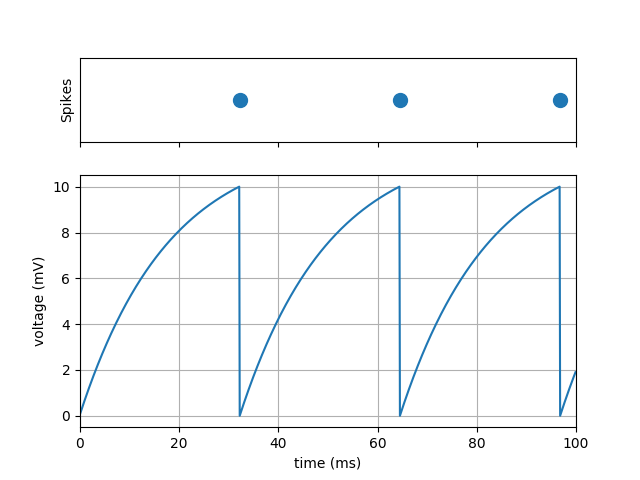
\includegraphics[width=.9\linewidth]{figures/graphs/singleSpikingNeuron.png}
        \caption{IF model}
        \label{fig:LIFSingleSpikeGraph}
    \end{subfigure}%
    \begin{subfigure}{.8\textwidth}
        \centering
        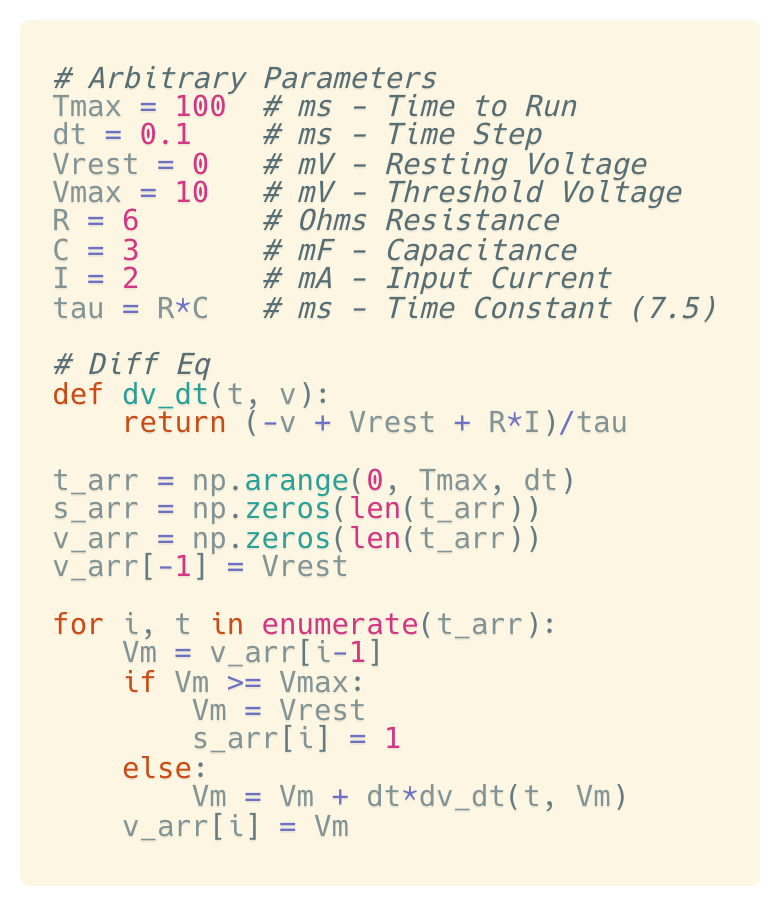
\includegraphics[width=.7\linewidth]{figures/code/SingleLIFCode.png}
        \caption{IF Currents}
        \label{fig:LIFCode}
    \end{subfigure}
    \DoubleCaption{Schematics of an Integrate and Fire model}{\small{Redrawn and
    adapted from \cite{gerstner_spiking_2002}}}
    \label{fig:LIFSingleSpikeGraphCode}
\end{figure}



% \begin{figure*}[h]
%     \centering

% \end{figure*}



% \begin{figure*}[h]
%     \centering
%     \begin{equation}\label{eq:LIF_TC}
%         T_C
%     \end{equation}
%     \begin{equation}\label{eq:LIF_RC}
%         \frac{d V}{d t} = -\frac{V}{\tau_L} + \frac{I(t)}{C}
%     \end{equation}
%     \begin{equation}\label{eq:integ_LIF_RC_VL}
%         V(t)= \frac{1}{C} \int_{0}^{t} e^{-\frac{(t-s)}{\tau_L}} I(s) ds
%     \end{equation}
%     $C$ is the membrane capacity, $g_L$ is the leak conductance and $V_L$ is the leak reversal potential.
%     % \caption{Formulae for a Leaky Integrate and Fire Neuron (pre-threshold)}
%     \label{LIFequation}
% \end{figure*}

\subsection{Spike refractory periods}

\subsection{STDP}